\documentclass[10pt,a4paper,ngerman]{scrartcl}
\usepackage[utf8]{inputenc}
\usepackage[ngerman]{babel}
\usepackage[T1]{fontenc}
\usepackage{amsmath}
\usepackage{amsfonts}
\usepackage{amssymb}
\usepackage{makeidx}
\usepackage{graphicx}
\usepackage{epstopdf}
\usepackage[onehalfspacing]{setspace}
\usepackage{array}
\usepackage{upgreek}
\usepackage{float}
\usepackage{csquotes}
\usepackage{chemformula}
\usepackage{chemgreek}
\usepackage{chemmacros}
\chemsetup{modules=all}
\usepackage{tikz}
\usepackage{siunitx}
\sisetup{locale = DE,per-mode = symbol}
\usepackage{esvect}
\usepackage{geometry}
\usepackage{pdfpages}
\usepackage[font=small]{caption}
%\usepackage[version=4]{mhchem}
\usepackage[backend=biber, style=chem-angew]{biblatex}
\addbibresource{Polyaddition_Polykond.bib}
\usepackage{tabularx, booktabs, multirow}
\usepackage[pdfborder={0 0 0}]{hyperref}
\usepackage{scrlayer-scrpage}%Header für die KOMA-script -Klasse
%\usepackage{hyperref}
\usepackage{pgfplots}
\usepackage{textgreek}


\newcommand{\tildenu}{{\fontencoding{LGR}\selectfont\accperispomeni\textnu}}
\captionsetup{format=plain}
\chemsetup[phases]{pos=sub}
\chemsetup[redox]{pos=top}
\chemsetup[redox]{align=center}
%\chemsetup[redox]{explicit-sign=true}
%\chemsetup[redox]{roman=false}
\newcommand{\celsius}{^{\circ}\mathrm{C}}
\parindent0pt
\sloppy
\DeclareChemPhase{\s}{s}
\DeclareChemPhase{\l}{l}
\DeclareChemPhase{\g}{g}
\renewcaptionname{ngerman}{\figurename}{Abb.}
\renewcaptionname{ngerman}{\tablename}{Tab.}
\geometry{bottom=100pt} \geometry{top=80pt}
\newcommand{\m}{\mathrm{m}}
\newcommand{\K}{\mathrm{K}}
\newcommand{\J}{\mathrm{J}}
\newcommand{\gr}{\mathrm{g}}
\newcommand{\kg}{\mathrm{kg}}
\newcommand{\mol}{\mathrm{mol}}
\newcommand{\Pa}{\mathrm{Pa}}
\newcommand{\ad}{\mathrm{ad}}
\newcommand{\de}{\mathrm{de}}
\newcommand{\gmol}{\mathrm{\frac{g}{mol}}}
\newcommand{\JKmol}{\mathrm{\frac{J}{K \cdot mol}}}
\newcommand{\kgmss}{\mathrm{\frac{kg}{m \cdot s^2}}}
\newcommand{\loge}{\mathrm{ln}}


\begin{document}
\begin{titlepage}
	\vspace*{2,5cm}
	\begin{center}
		\begin{LARGE}
			\textbf{Polymer Chemie}\\
			\textbf{Radikalische (Co)Polymerisation}\\
		\end{LARGE}
		\vspace{1cm}
		\textbf{Universität Stuttgart}\\
		\vspace*{1,5cm}
		\begin{tabular}{lp{7,5cm}l}
			Author 1:     &Laurens Viehoff\\
            Author 2:     &Felix Roth\\   
			E-Mail 1:      &st183688@stud.uni-stuttgart.de\\
            E-Mail 2:      &st188157@stud.uni-stuttgart.de  \\
			Student-ID 1: & 3676761   \\ 
            Student-ID 2: & 3711192 \\ \\
			Assistentin:  &   \\ \\ 
		\end{tabular}
	\end{center}

    
\end{titlepage}
\thispagestyle{empty}
\renewcommand{\thepage}{\arabic{page}}
\newpage
\tableofcontents
\setcounter{page}{1}
\renewcommand{\thepage}{\arabic{page}}
\newpage


\section{Theorie}

	Im allgemeinen lässt sich die radikalische Polymerisation in drei Teilschritte einteilen.
	Der erste Schritt ist der Kettenstart, hierbei wird mittels eines radikalstarters (im falle des Versuchs AIBN), thermisch ein Radikal gebildet (\ref{Kettenstart}).

	
		\begin{figure}[H]
			\centering
			
\includegraphics[scale = 0.25]{Bilder/Initiierung.png}
			\caption{}
			\label{Kettenstart}
		\end{figure}

	Dieses gebildete Radikal greift radikalisch an dem vinylischen Kohlenstoff an.
	Dabei entsteht das Radikal an der benzylischen Stelle.
	Wichtig ist jedoch, dass nicht alle Radikale des Initiators an der Polymerisation beteiligt sind.
	Dafür lässt sich der Radikal-Ausbeute-Faktor $f$ bestimmen.
		
		\begin{equation}
			f = \frac{\sum \text{kettenstart}R^*}{\sum \text{gebildete}R^*}
			\label{Cage-Effekt}
		\end{equation}
	
	Der zweite Schritt besteht aus dem Kettenwachstum. Hierbei wird die Polymerkette mittels weiterem Monomer gebildet.

	%chemDraw

	Für diesen Schritt lässt sich ein Zeitgesetzt aufstellen welches die wachstums Geschwindigkeit $v_w$ und die Geschwindigkeitskonstante $k_w$ berücksichtigen.
	
		\begin{equation}
			v_w = k_w [p^*][M]
			\label{Zeitgesetzt}
		\end{equation}

	Der letzte und dritte Schritt ist der Abbruchsschritt. Bei diesem gibt es zwei möglichkeiten eines Abbruchs.
	Der erste wäre die Rekombination auch in Abb. xxx gezeigt. Hierbei reagieren zwei Radikale miteinander und bilden eine Bindung aus. 
	Das reaktive Radikal geht somit verloren.\\ 
	Die andere Variante wäre eine Disproportionierung hierbei findet wie in Abb. [xxx] gezeigt eine Radikalische bindung zwischen einem Monomer und dem $\alpha$-Wasserstoff statt. 
	Dabei findet zusätzlich eine Rekombination zu einer Doppelbindung statt. 
	
	
	%Vielleicht Gleichung


	Desweiteren kann der Umsatz in abhängigkeit zu dem Polymerisationsgrad aufgetragen werden, wordurch folgender Graph entsteht.

		\begin{figure}[H]
			\centering
			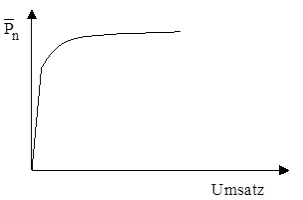
\includegraphics[scale = 0.7]{Bilder/GraphPG.png}
			\caption{Die Abbildung beschreibt die Abhängigkeit des Polymerisationsgrad vom Umsatz. \cite{polyskript}}
			\label{GraphPG}
		\end{figure}

	Für diese Kinetik spielt auch das sogenannte "Wurzel-I-Gesetz" eine große Rolle. 
		
	Um dieses Aufstellen zu können wird unteranderem von sechs Annahmen ausgegangen.\\
	
	Die erste ist, dass vorhandensein einer irreversieblen Reaktion.\\
	
	Die zweite ist, dass die Initiatorradikal-konzentration stationär ist. 
	Was soviel bedeutet wie, gleich viele Radikale werden durch zerfall des Initiators gebildet wie verbraucht werden.\\

	Die dritte Beschreibt, dass die Initiatorkonzentration während der Polymerisation konstant bleibt.\\

	Die vierte beschreibt im großen und ganzen, dass die Bruttoreaktionsgeschwindigkeit $v_\text{Br}$ und die Wachstumsreaktionsgeschwindigkeit $v_w$ gleich sind woduch folgt:

		\begin{equation}
			v_\text{Br} \approx v_w = k_w [P^*][M]
		\end{equation}

	Die fünfte, ist das ausgehen von einem Abbruch welcher lediglich durch gegenseitige Desaktivierung der Polymere erfolgt.\\

	Die sechste und letzte ist ähnlich wie die zweite nur das davon ausgegangen wird, dass die Polymerradikal-konzentration stationer ist.\\

	Das Wurzel-I-Gesetz definiert die Bruttoreaktionsgeschwindigkeit und ist in Gleichung \ref{WurzelI} beschrieben

		\begin{equation}
			v_\text{Br} = k_w \sqrt{\frac{2k_z f}{k_{ab}}\sqrt{[I]}[M]}
			\label{WurzelI}
		\end{equation}

	Um diese Geschwindigkeiten zu bestimmen werden Eigenschaften wie Volumen der Polymerlösung, 
	abnahme der Monomerkonzentration oder die Zunahme der Polymermenge verwendet. 
	Desweiteren ist die Bruttogeschwindigkeit abhängig von der Konzentration der Edukte.\\

	Allgemein wird um die güte einer Polymerisation zu bestimmen der zahlenmittlere Polymerisationsgrad bestimmt. 
	Dieser wird in zwei unterschiedlichen Formeln beschrieben wobei Formel (\ref{Pn1}) den Polymerisationsgrad bei abbruch durch Kombination beschreibt, 
	und Formel (\ref{Pn2}) den Polymerisationsgrad bei Kettenabruch durch Disproportionierung beschreibt.

		\begin{equation}
			P_n = 2v\\
			\label{Pn1}
		\end{equation}

		\begin{equation}
			P_n = v
			\label{Pn2}
		\end{equation}
		
	
	
	

\printbibliography

\end{document}